\section{Analysis}
\label{sec:Analysis}

Before working with the actual data, a simulation sample is used to familiarize oneself with the structure of the data. This simulation sample includes only $B^\pm$ candidates decaying into three Kaons. The distributions of the momenta belonging to the first Kaon is shown in \autoref{fig:momentum}. 

\begin{figure}
	\centering
	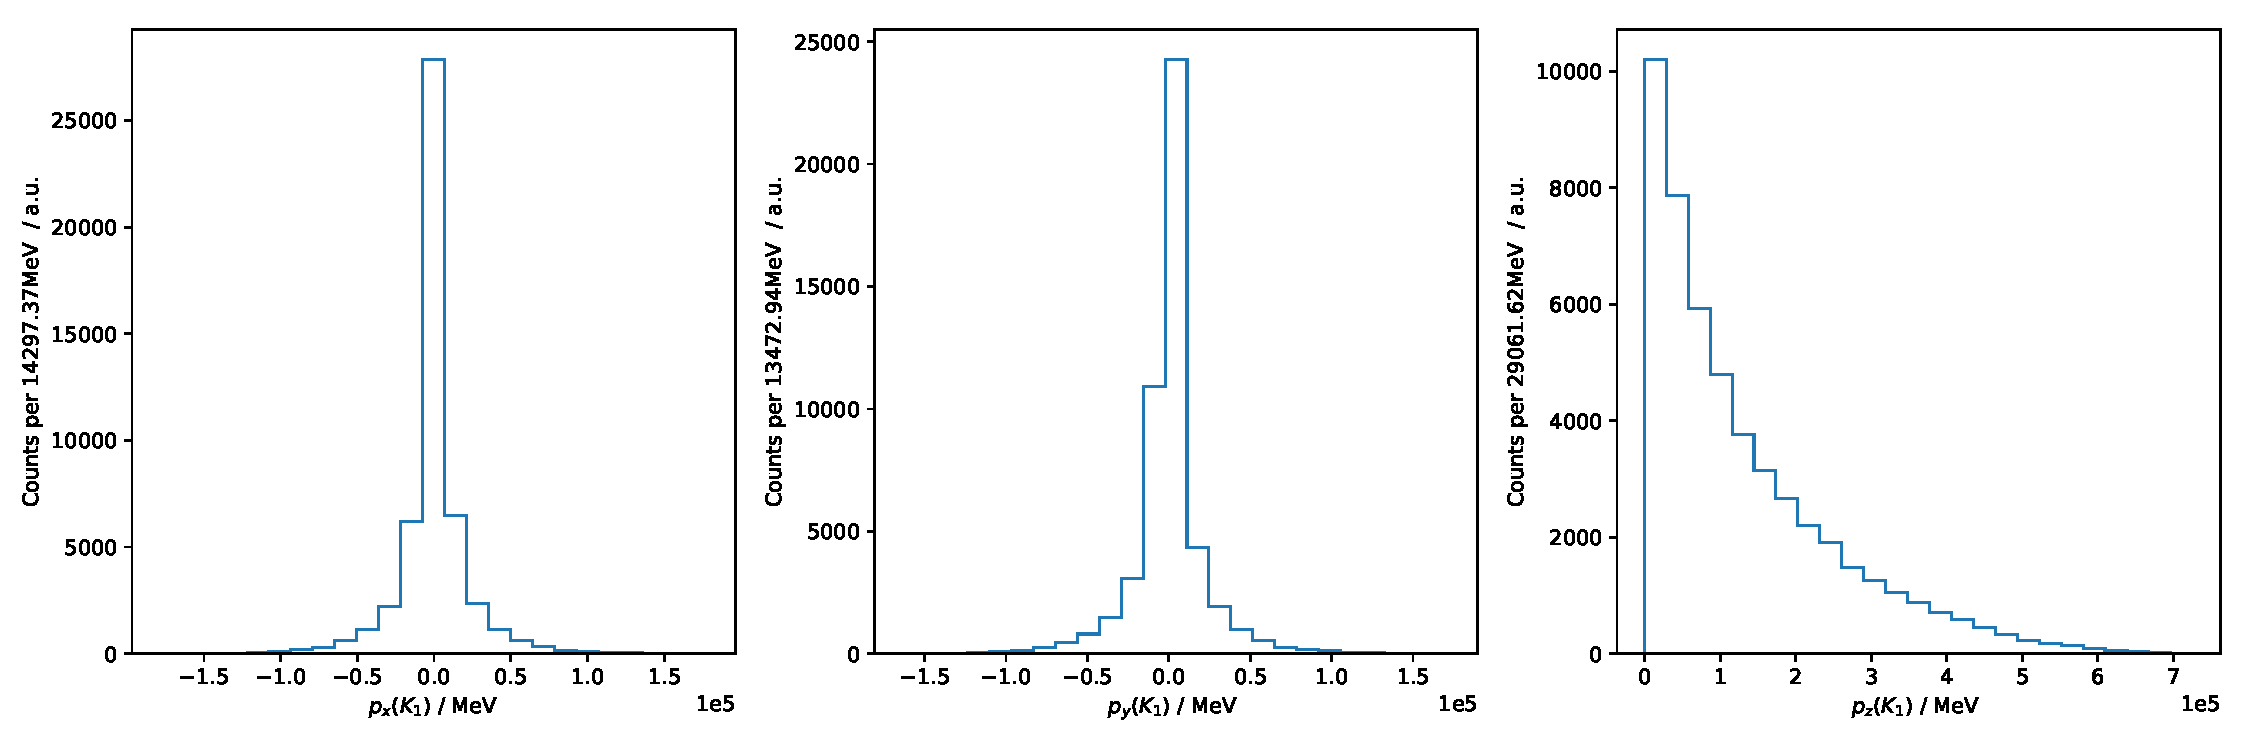
\includegraphics[width=0.9\linewidth]{content/pictures/image_fin/momentum}
	\caption{Momentum distributions of the fist Kaon.}
	\label{fig:momentum}
\end{figure}


From the momenta and the nominal mass of the Kaon $m(K^\pm) = \qty{493.677 \pm 0.015}{\mega\eV }$  the energy carried by the Kaon is determined \cite{pdg}. The Energy distribution is shown in \autoref{fig:energyk1}

\begin{figure}
	\centering
	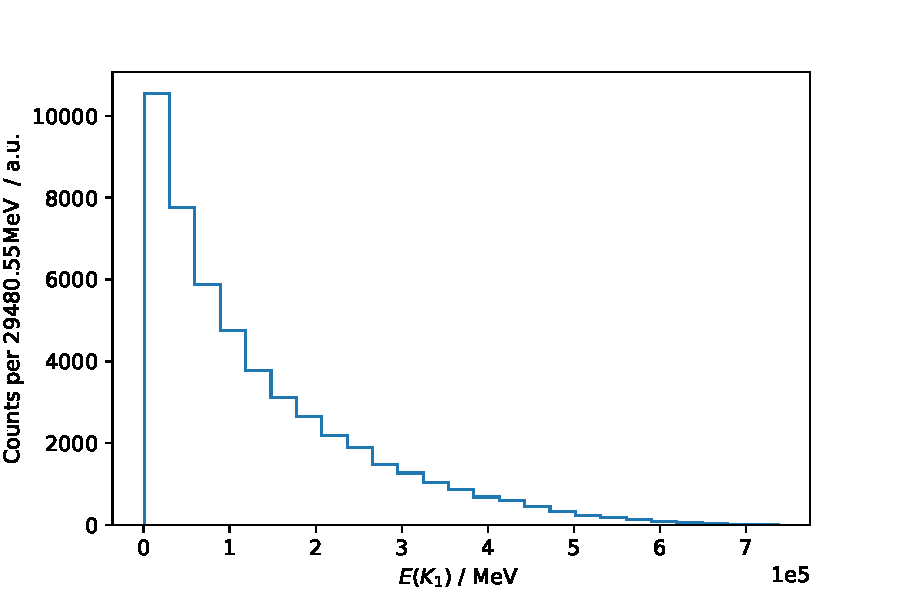
\includegraphics[width=0.6\linewidth]{content/pictures/image_fin/energyK1}
	\caption{Histogram of the energy determined form the fist Kaons momenta.}
	\label{fig:energyk1}
\end{figure}


Using the determined energy and momenta of the Kaons the four momenta of the $B^\pm$ can be calculated. The four moment are then used to determine the invariant mass of the $B^\pm$. This distribution is not shown as the peak around the nominal mass $m(B^\pm) = \qty{5279.41\pm0.07}{\mega\eV}$ is to narrow for histogramming \cite{pdg}. \\


Before working with the data sample an additional requirement is placed on the \texttt{prob} variables to ensure the studied candidates are originating from the $B^\pm \rightarrow K^+ K^- K^\pm$ decay. This requirement is applied, because the data sample contains candidates form additional decays, e.g. including Pions. The values for the requirement on the candidates determined probability are chosen to be: 
\begin{align}
	\mathtt{H1\_probK} &> 0.5\\
	\mathtt{H1\_probPi} &< 0.5
\end{align}

The same steps explained for the simulation sample are then performed on the data sample in order to obtain the $B$-Mesons invariant mass distribution, shown in \autoref{fig:invmass}. 

\begin{figure}
	\centering
	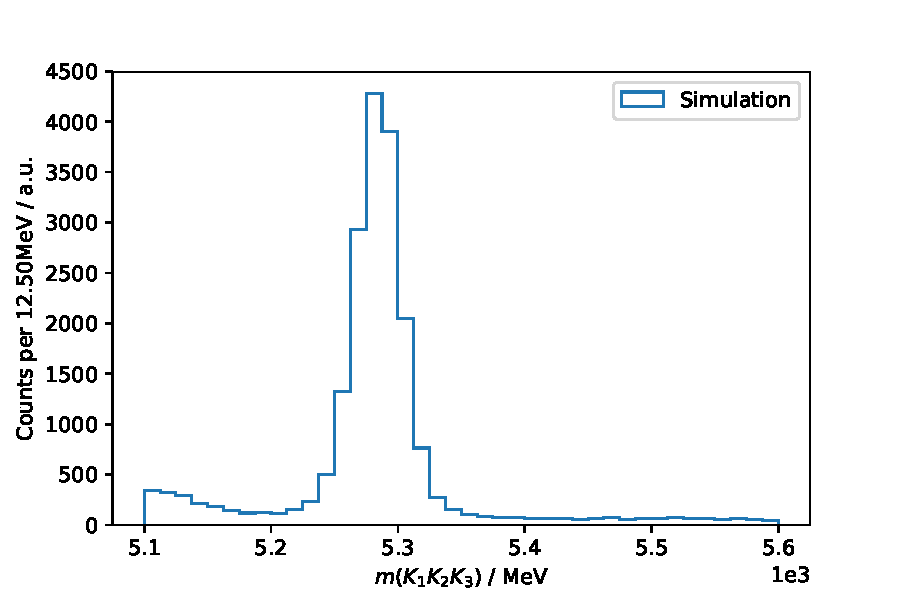
\includegraphics[width=0.7\linewidth]{content/pictures/image_fin/invmass}
	\caption{Invariant mass distribution of the $B^\pm$.}
	\label{fig:invmass}
\end{figure}
In 

In order to calculate the global $CP$-asymmetry $A_\mathrm{CP}$ the signal counts of the $B^+$ and $B^-$ have to be determined. This is achieved by fitting the function 
\begin{equation}
	f(x) = N\exp\left(-\lambda x\right) + A  \exp\left(\frac{(x-\mu)^2}{2\sigma^2}\right)
	\label{eq:fit}
\end{equation} 
onto the counts determined from a histogram and calculating the signal counts as the area under the gaussian function $\sqrt{2\pi}A\sigma$. The plots of the fitted data for both $B^+$ and $B^-$ candidates are given \autoref{fig:fits}


\begin{figure}[H]
	\centering
	\begin{subfigure}{0.45\textwidth}
		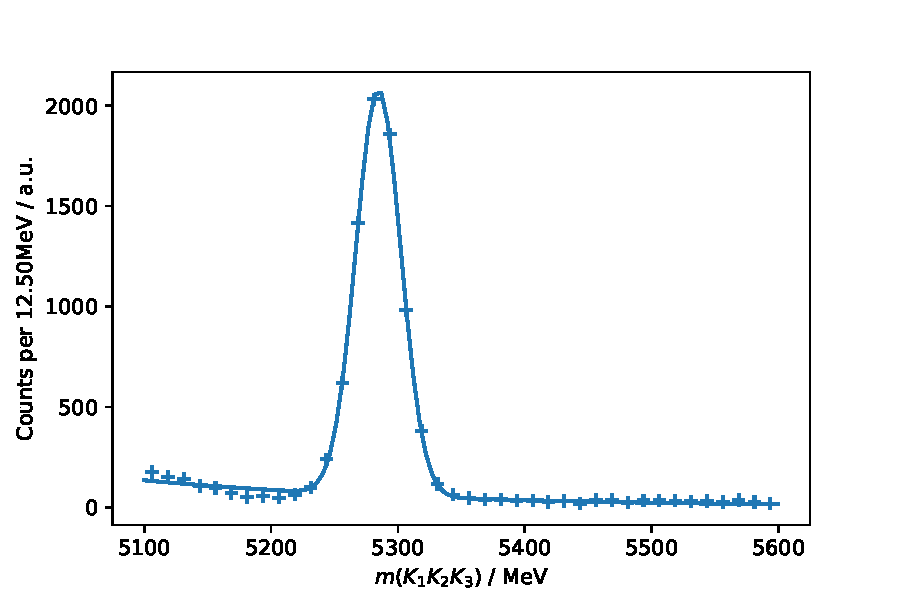
\includegraphics[width=\textwidth]{content/pictures/image_fin/invmassFitBN.pdf}
		\caption{$B^+$}
	\end{subfigure}
	\begin{subfigure}{0.45\textwidth}
		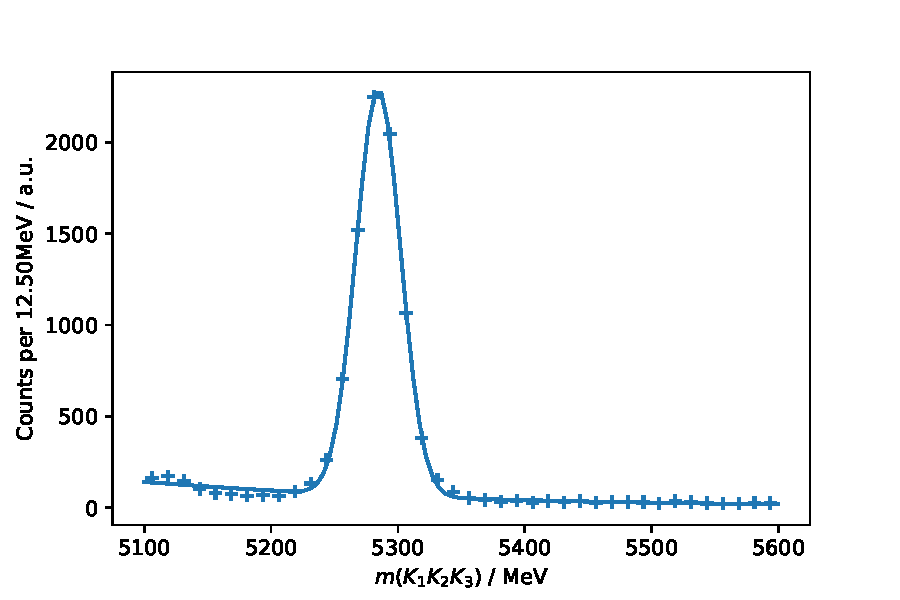
\includegraphics[width=\textwidth]{content/pictures/image_fin/invmassFitBP.pdf}
		\caption{$B^-$}
	\end{subfigure} 
	\caption{Function \autoref{eq:fit} fitted on the counts determined from the histograms of both $B^+$ and $B^-$ candidates.}
	\label{fig:fits}
\end{figure}


